% Created 2025-06-23 ma 17:46
% Intended LaTeX compiler: pdflatex
\documentclass[11pt]{article}
\usepackage[mathletters]{ucs}
\usepackage[utf8x]{inputenc}
\usepackage[T1]{fontenc}
\usepackage{graphicx}
\usepackage{longtable}
\usepackage{wrapfig}
\usepackage{rotating}
\usepackage[normalem]{ulem}
\usepackage{amsmath}
\usepackage{amssymb}
\usepackage{capt-of}
\usepackage{hyperref}
\usepackage{minted}
\author{Jan Boone}
\date{\today}
\title{}
\hypersetup{
 pdfauthor={Jan Boone},
 pdftitle={},
 pdfkeywords={},
 pdfsubject={},
 pdfcreator={},
 pdflang={English}}
\begin{document}

We consider a situation where the government wants to invest in a public good financed by an income tax. The cost of the project is 18k (per head) and the question is whether the tax raised by a nonlinear income tax schedule will be enough to cover the cost. We estimate the parameters of the (Pareto) income distribution and then see whether the expected tax income exceeds the cost.

Due to the nonlinearity of the tax scheme, it is hard to propagate the parameter uncertainty into the uncertainty of the tax revenue using a frequentist approach. With a Bayesian analysis this is straightforward to do: we feed the posterior distribution of the parameters into the tax function.

Another advantage of Bayesian analysis is that one can do a scenario analysis, say the cost of the project can be low, average or high with certain probabilities.

We first generate a sample from the theoretical income distribution. With this sample of 50 individuals, we will estimate the parameters of our model.


\begin{minted}[]{python}
import numpy as np
import pymc as pm
from pymc import do, observe
N=50
individuals = np.arange(N)

with pm.Model(coords={"individuals":individuals}) as model_income:
    alpha = pm.HalfNormal("alpha",1)
    m = pm.Normal("m",30000,5000)
    income = pm.Pareto('income', alpha=alpha, m=m,dims="individuals")


true_values = {
    "alpha": 3.0,
    "m": 30000
}

income_simulate = do(model_income, true_values)

with income_simulate:
    simulate = pm.sample_prior_predictive(samples=1)


income_data = simulate.prior.income.values
# income_data
\end{minted}

\phantomsection
\label{}
\begin{verbatim}
Sampling: [income]
\end{verbatim}



Given the \texttt{income\_data}  that we have, the following code block generates the posterior distribution of the parameters \(\alpha,m\).

\begin{minted}[]{python}
model_inference = observe(model_income,\
                {"income":income_data[0,0]})

with model_inference:
    idata = pm.sample(progressbar=False)

\end{minted}

\phantomsection
\label{}
\begin{verbatim}
Initializing NUTS using jitter+adapt_diag...
Multiprocess sampling (4 chains in 4 jobs)
NUTS: [alpha, m]
Sampling 4 chains for 1_000 tune and 1_000 draw iterations (4_000 + 4_000 draws total) took 2 seconds.
There were 2808 divergences after tuning. Increase `target_accept` or reparameterize.
The rhat statistic is larger than 1.01 for some parameters. This indicates problems during sampling. See https://arxiv.org/abs/1903.08008 for details
The effective sample size per chain is smaller than 100 for some parameters.  A higher number is needed for reliable rhat and ess computation. See https://arxiv.org/abs/1903.08008 for details
\end{verbatim}


We can view the estimates and the values for \texttt{r\_hat}.

\begin{minted}[]{python}
import arviz as az
headers = ['mean', 'sd', 'hdi_3%', 'hdi_97%',\
           'ess_bulk', 'r_hat']
variables = ["m","alpha"]
df_summary = az.summary(idata,var_names=variables)[headers]
df_summary
\end{minted}

\phantomsection
\label{}
\begin{verbatim}
            mean       sd     hdi_3%    hdi_97%  ess_bulk  r_hat
m      29933.492  239.609  29513.609  30166.580     310.0   1.01
alpha      2.658    0.359      1.963      3.297     564.0   1.00
\end{verbatim}



Next we generate our posterior predictive distribution of income. This is our posterior distribution of the income distribution (with the uncertainty of our parameters incorporated). In other words, this is our best guess of the income distribution that we will use to get an idea of the tax revenues that the government can expect.

\begin{minted}[]{python}
idata_posterior_predictive = pm.sample_posterior_predictive(idata,model=model_inference,progressbar=False)
posterior_predictive_incomes = idata_posterior_predictive.posterior_predictive.income.values
\end{minted}

\phantomsection
\label{}
\begin{verbatim}
Sampling: [income]
\end{verbatim}


The following code block defines the nonlinear tax function. And we calculate the posterior distribution for the tax revenue.

\begin{minted}[]{python}
import pytensor
import pytensor.tensor as pt


def piecewise_linear_tax_scalar(income, thresholds, rates):
    """
    Calculates the tax for a given income based on a piecewise linear tax function.
    This function works for inputs of any dimension due to broadcasting.
    """
    t1, t2 = thresholds
    r1, r2, r3 = rates

    # Tax for the first bracket
    tax = np.minimum(income, t1) * r1

    # Tax for the second bracket
    tax += np.maximum(0, np.minimum(income, t2) - t1) * r2

    # Tax for the third bracket
    tax += np.maximum(0, income - t2) * r3

    return tax

def piecewise_linear_tax(income, thresholds, rates):
    """
    Calculates the tax for a given income based on a piecewise linear tax function.
    This function works for inputs of any dimension due to broadcasting.
    """
    t1, t2 = thresholds
    r1, r2, r3 = rates

    # Tax for the first bracket
    tax = pt.minimum(income, t1) * r1

    # Tax for the second bracket
    tax += pt.maximum(0, pt.minimum(income, t2) - t1) * r2

    # Tax for the third bracket
    tax += pt.maximum(0, income - t2) * r3

    return tax


# pt.dtensor3 creates a placeholder for a 3D tensor with double-precision floats.
income_tensor_3d = pt.dtensor3('income_3d')

# Define the realistic parameters for the Netherlands (2025 system)
thresholds = (38441, 76817)
rates = (0.3582, 0.3748, 0.4950)

tax_due_3d = piecewise_linear_tax(income_tensor_3d, thresholds, rates)
calculate_tax_3d = pytensor.function(inputs=[income_tensor_3d], outputs=tax_due_3d)

# Use the compiled function to calculate the taxes
tax_income_per_head = calculate_tax_3d(posterior_predictive_incomes)

tax_income_per_head.shape
\end{minted}

\begin{table}[htbp]
\label{}
\centering
\begin{tabular}{rrr}
4 & 1000 & 50\\
\end{tabular}
\end{table}


In a frequentist approach one can calculate the expected tax revenue. This expectation may (or may not) differ significantly from the target of 18k needed to finance the public good. Whether or not it does, what do we learn from this?

\begin{minted}[]{python}
tax_income_per_head.mean(axis=2).mean(), tax_income_per_head.mean(axis=2).std()
\end{minted}

\begin{table}[htbp]
\label{}
\centering
\begin{tabular}{rr}
18336.024427944103 & 3549.055002477104\\
\end{tabular}
\end{table}

The Bayesian approach allows us to quantify the uncertainty. The following figure shows 4 different distributions of the tax revenue. This figure shows that whether or not the mean tax revenue is above or below 18k is hardly relevant.

\begin{minted}[]{python}
import matplotlib.pyplot as plt
import seaborn as sns

# Assuming your tensor is called 'data_tensor'
data = tax_income_per_head.mean(axis=2)  # Convert to numpy array if using PyTorch

for i in range(4):
    sns.kdeplot(data[i, :])

plt.axvline(x=tax_income_per_head.mean(), color='black', linestyle='--',label="expected tax revenue per head")  # Add vertical line
# plt.axvline(x=piecewise_linear_tax_scalar(posterior_predictive_incomes.mean(),thresholds,rates), color='blue', linestyle=':',label="tax of expected income per head")  # 
plt.legend()
plt.xlim(0,50000)
plt.xlabel("tax revenue per head")
plt.suptitle('Four posterior distributions of tax revenue per head')
plt.tight_layout();

\end{minted}

\begin{center}
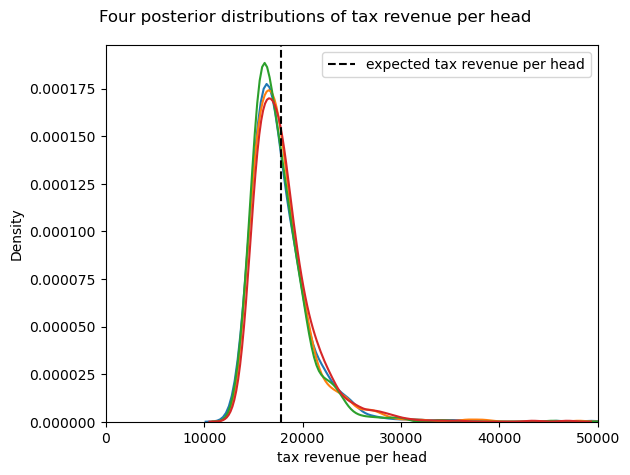
\includegraphics[width=.9\linewidth]{./figures/average_tax_income_distributions.png}
\label{}
\end{center}


With the Bayesian approach we can answer the question: how likely is it that tax revenue falls below the 18k threshold:

\begin{minted}[]{python}
threshold = 18000
print(data.mean())
print(np.mean(data < threshold))
\end{minted}

\phantomsection
\label{}
\begin{verbatim}
18336.024427944103
0.57575
\end{verbatim}



We can make a graph to show how the probability of earning enough tax revenues varies with the top tax rate that we use.

\begin{minted}[]{python}
import pytensor
import pytensor.tensor as pt
import numpy as np

def calculate_revenue_for_top_rates(income_tensor, top_rates_var, thresholds, base_rates):
    """
    Calculates the total tax revenue for a tensor of incomes across a vector of
    variable top tax rates.
    """
    t1, t2 = thresholds
    r1, r2 = base_rates

    # --- Broadcasting ---
    income = income_tensor.dimshuffle('x', 0, 1, 2)
    top_rates_reshaped = top_rates_var.dimshuffle(0, 'x', 'x', 'x')

    # --- Tax Calculation with Broadcasting ---

    # Tax for the first bracket. This part is constant for all top rates.
    tax = pt.minimum(income, t1) * r1

    # Tax for the second bracket. Also constant.
    tax += pt.maximum(0, pt.minimum(income, t2) - t1) * r2

    # Tax for the third bracket. This is where the broadcasting happens.
    tax += pt.maximum(0, income - t2) * top_rates_reshaped

    return tax

# --- Step 1: Define symbolic tensors ---

income_tensor_3d = pt.dtensor3('income_3d')
# A vector for the variable top tax rates
top_rates_vector = pt.dvector('top_rates')

# --- Step 2: Define fixed and variable parameters ---

# Fixed parameters
thresholds = (38441, 76817)
base_rates = (0.3582, 0.3748) # r1 and r2

# Variable parameter: A range of top tax rates (r3) to test
top_rates_range = np.linspace(0.45, 0.95, num=20) # Test 20 rates from 45% to 95%

# --- Step 3: Build the computation graph ---
revenue_graph = calculate_revenue_for_top_rates(
    income_tensor_3d,
    top_rates_vector,
    thresholds,
    base_rates
)

# --- Step 4: Compile the graph into a callable Python function ---
calculate_revenue = pytensor.function(
    inputs=[income_tensor_3d, top_rates_vector],
    outputs=revenue_graph
)

# Use the compiled function to calculate the revenues
calculated_revenues = calculate_revenue(posterior_predictive_incomes, top_rates_range)

\end{minted}

\begin{minted}[]{python}
data = calculated_revenues.mean(axis=3)
probabilities = np.mean(data >= threshold,axis=(1,2))
\end{minted}

The following figure shows how the probability of being able to finance the public good varies with the top tax rate. The higher this tax rate, the higher the probability that we generate enough tax revenues to cover the public good.

\begin{minted}[]{python}
plt.plot(top_rates_range,probabilities)
plt.xlabel('top tax rate')
plt.ylabel('probability')
plt.title('Probability that enough tax revenue is raised to pay for public good');
\end{minted}

\begin{center}
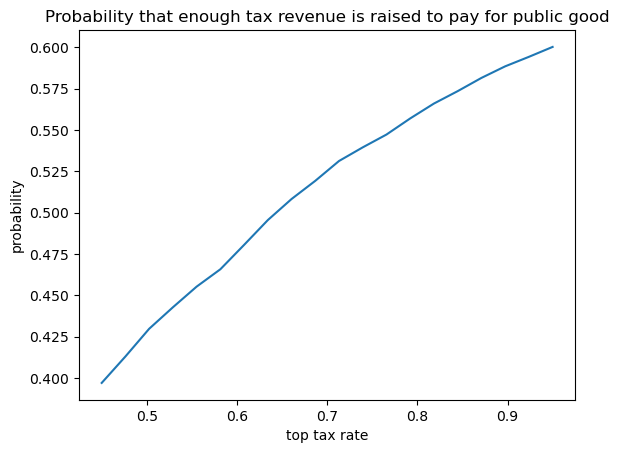
\includegraphics[width=.9\linewidth]{./figures/probabilities.png}
\label{}
\end{center}
\end{document}
